\begin{appendix}
    \chapter*{Appendices}
    \label{cha:appendices}
    \addcontentsline{toc}{chapter}{Appendices}

    % \includeappendixpdfwithtitle{Task Description from Norkart}{appendices/project_description.pdf}{app:task-description}

    % \chapter{Datasets}
    % \label{app:datasets}
    % \begin{longtable}{p{3cm}p{2cm}p{5.7cm}p{2.5cm}}
    \caption{Datasets used in the experiments}                                                                                                                                                                                                              \\
    \label{tbl:datasets}                                                                                                                                                                                                                                    \\
    \toprule
    \textbf{Dataset}   & \textbf{Type} & \textbf{Description}                                                                                                                                                                         & \textbf{\#Features} \\
    \midrule
    \endfirsthead

    \multicolumn{4}{c}{{\bfseries Table \thetable\ continued from previous page}}                                                                                                                                                                           \\
    \toprule
    \textbf{Dataset}   & \textbf{Type} & \textbf{Description}                                                                                                                                                                         & \textbf{\#Features} \\
    \midrule
    \endhead

    \midrule
    \multicolumn{4}{r}{Continued on next page}                                                                                                                                                                                                              \\
    \midrule
    \endfoot

    \bottomrule
    \endlastfoot

    Buildings          & Polygon       & Contains building outlines. Its \emph{type} attribute can have values like \enquote{house}, \enquote{university}, and \enquote{restaurant}.                                                  & 4,147,645           \\
    Land Use           & Polygon       & Represents areas designated to different purposes and activities. Its \emph{fclass} attribute can have values like \enquote{forest}, \enquote{farmland}, and \enquote{residential}.          & 541,452             \\
    Natural            & Point         & Contains outlines of various objects found in nature. Its \emph{fclass} attribute can have values like \enquote{beach}, \enquote{glacier}, and \enquote{cave\_entrance}.                     & 119,725             \\
    Natural            & Polygon       & Similar to the point data equivalent.                                                                                                                                                        & 6,665               \\
    Places of Worship  & Point         & Common values for \emph{fclass} attribute: \enquote{christian}, \enquote{buddhist}, and \enquote{muslim}.                                                                                    & 311                 \\
    Places of Worship  & Polygon       & Similar to the point data equivalent.                                                                                                                                                        & 2,520               \\
    Places             & Point         & Common values for \emph{fclass} attribute: \enquote{farm}, \enquote{village}, and \enquote{island}.                                                                                          & 178,997             \\
    Places             & Polygon       & Similar to the point data equivalent.                                                                                                                                                        & 5,689               \\
    Points of Interest & Point         & Common values for \emph{fclass} attribute: \enquote{tourist\_info}, \enquote{bench}, and \enquote{kindergarten}.                                                                             & 117,677             \\
    Points of Interest & Polygon       & Similar to the point data equivalent.                                                                                                                                                        & 45,825              \\
    Railways           & Line          & Common values for \emph{fclass} attribute: \enquote{rail}, \enquote{subway}, and \enquote{tram}. Also has True/False attributes \emph{bridge} and \emph{tunnel}.                             & 14,008              \\
    Roads              & Line          & Common values for \emph{fclass} attribute: \enquote{rail}, \enquote{subway}, and \enquote{tram}. Has additional attributes \emph{oneway}, \emph{maxspeed}, \emph{bridge}, and \emph{tunnel}. & 1,741,929           \\
    Traffic            & Point         & Common values for \emph{fclass} attribute: \enquote{crossing}, \enquote{street\_lamp}, and \enquote{parking}.                                                                                & 98,860              \\
    Traffic            & Polygon       & Common values for \emph{fclass} attribute: \enquote{parking}, \enquote{pier}, and \enquote{dam}.                                                                                             & 45,623              \\
    Transport          & Point         & Common values for \emph{fclass} attribute: \enquote{bus\_stop}, \enquote{ferry\_terminal}, and \enquote{railway\_station}.                                                                   & 91,627              \\
    Transport          & Polygon       & Similar to the point data equivalent.                                                                                                                                                        & 935                 \\
    Water              & Polygon       & Common values for \emph{fclass} attribute: \enquote{water}, \enquote{wetland}, and \enquote{river\_bank}.                                                                                    & 1,861,199           \\
    Waterways          & Line          & Common values for \emph{fclass} attribute: \enquote{stream}, \enquote{river}, and \enquote{canal}.                                                                                           & 833,253             \\
\end{longtable}



    \chapter{Experiments}
    \label{app:experiments}

    \section[GIS Benchmark Experiment]{\acrshort{acr:gis} Benchmark Experiment}
    \label{appsec:questions-and-answer}

    \begin{longtable}{p{4cm}p{4.5cm}p{4.5cm}}
\caption{Questions for GIS benchmark experiment} \label{tbl:questions-quantitative} \\
\toprule
\textbf{Query} \textbf{ID} & \textbf{Query} & \textbf{Correct} \textbf{Response} \\
\midrule
\endfirsthead
\caption[]{Questions for GIS benchmark experiment} \\
\toprule
\textbf{Query} \textbf{ID} & \textbf{Query} & \textbf{Correct} \textbf{Response} \\
\midrule
\endhead
\midrule
\multicolumn{3}{r}{Continued on next page} \\
\midrule
\endfoot
\bottomrule
\endlastfoot
aker\_brygge\_national & Which is the closest railway station to Aker brygge? & Nationalteateret \\
cliff\_clusters & Locate clusters of cliffs, each containing more than 10 cliffs, with cliffs within each cluster no more than 0.1 degrees apart. & Should be about 8-9 clusters.  \\
county\_names & What are the names of the counties in found in the data? & Nordland, Telemark, Troms, Rogaland, Vestland, Trøndelag, Vestfold, Buskerud, Akershus, Østfold, Innlandet, Møre og Romsdal, Agder Finnmark \\
glomma\_counties & How many counties does Glomma run through? & 4. Trøndelag, Innlandet, Akershus, and Østfold.  \\
largest\_county  & Which is the largest county by size? & Nordland \\
nidarosdomen\_polygon & Retrieve a polygon of Nidarosdomen.  & Adding a polygon of Nidarosdomen to the map. \\
num\_trees\_munkegata & How many trees are there along Munkegata in Trondheim? & Giving the correct number of trees (about 70-80). \\
oslo\_bergen\_geodesic & Create a geodesic curve between the airports of Oslo and Bergen.  & A geodesic, slightly curved line between Gardermoen and Flesland. \\
oslo\_residental\_diff & Provide an outline of Oslo but exclude residential areas by computing their difference. & The polygonal outline of Oslo with cutouts where there area areas classified as residental.  \\
oslo\_roads\_gte\_70\_kmh & Retrieve roads in Oslo that have speed limit higher than or equal to 70 km/h.  & Adding corresponding line segments to the map. \\
vestfold\_bbox & Find the coordinates that define a the extent of a rectangular bounding box that encompasses the county of Vestfold. & (9.7553357, 58.720455, 10.6750198, 59.674011) \\
viken\_dissolve & Combine the countries that correspond to the historical country of Viken into a single feature.  & Display the outline of Viken, based on the outlines of Buskerud, Aksershus, and Østfold, that are found in the data. Should be dissolved, i.e., no borders.  \\
\end{longtable}

    \newpage
    \begin{longtable}{lp{1.8cm}p{1.8cm}p{1.8cm}p{1.8cm}p{1.8cm}}
    \caption{Results from GIS benchmark experiment} \label{tbl:test-results-quantitative}                                          \\
    \toprule
    \textbf{Query} \textbf{ID} & \textbf{Agent} \textbf{Type} & \textbf{Outcome} & \textbf{Latency} [\textbf{s}] & \textbf{Tokens} \\
    \midrule
    \endfirsthead
    \caption[]{Results from GIS benchmark experiment}                                                                              \\
    \toprule
    \textbf{Query} \textbf{ID} & \textbf{Agent} \textbf{Type} & \textbf{Outcome} & \textbf{Latency} [\textbf{s}] & \textbf{Tokens} \\
    \midrule
    \endhead
    \midrule
    \multicolumn{5}{r}{Continued on next page}                                                                                     \\
    \midrule
    \endfoot
    \bottomrule
    \endlastfoot
    aker\_brygge\_national     & oaf                          & partial success  & 87.16                         & 3347            \\
    aker\_brygge\_national     & oaf                          & partial success  & 97.85                         & 3042            \\
    aker\_brygge\_national     & oaf                          & partial success  & 70.36                         & 4563            \\
    aker\_brygge\_national     & python                       & partial success  & 68.10                         & 4736            \\
    aker\_brygge\_national     & python                       & partial success  & 49.48                         & 2192            \\
    aker\_brygge\_national     & python                       & partial success  & 76.84                         & 4270            \\
    aker\_brygge\_national     & sql                          & success          & 63.51                         & 2569            \\
    aker\_brygge\_national     & sql                          & success          & 151.46                        & 6273            \\
    aker\_brygge\_national     & sql                          & success          & 103.98                        & 5169            \\
    cliff\_clusters            & oaf                          & partial success  & 93.21                         & 3047            \\
    cliff\_clusters            & oaf                          & partial success  & 134.62                        & 3713            \\
    cliff\_clusters            & oaf                          & failure          & 253.77                        & 6956            \\
    cliff\_clusters            & python                       & failure          & 66.42                         & 5421            \\
    cliff\_clusters            & python                       & failure          & 125.96                        & 4650            \\
    cliff\_clusters            & python                       & failure          & 109.29                        & 4768            \\
    cliff\_clusters            & sql                          & failure          & 39.36                         & 1633            \\
    cliff\_clusters            & sql                          & failure          & 75.27                         & 3085            \\
    cliff\_clusters            & sql                          & success          & 31.64                         & 1632            \\
    county\_names              & oaf                          & success          & 78.08                         & 2389            \\
    county\_names              & oaf                          & success          & 67.45                         & 2399            \\
    county\_names              & oaf                          & failure          & 20.23                         & 1471            \\
    county\_names              & python                       & success          & 44.33                         & 2532            \\
    county\_names              & python                       & success          & 30.50                         & 2355            \\
    county\_names              & python                       & success          & 31.09                         & 2355            \\
    county\_names              & sql                          & success          & 64.21                         & 1874            \\
    county\_names              & sql                          & success          & 52.28                         & 1880            \\
    county\_names              & sql                          & success          & 47.62                         & 1886            \\
    glomma\_counties           & oaf                          & success          & 69.73                         & 2253            \\
    glomma\_counties           & oaf                          & success          & 65.57                         & 1945            \\
    glomma\_counties           & oaf                          & success          & 67.37                         & 2397            \\
    glomma\_counties           & python                       & success          & 663.22                        & 3658            \\
    glomma\_counties           & python                       & failure          & 295.93                        & 4388            \\
    glomma\_counties           & python                       & success          & 285.23                        & 2281            \\
    glomma\_counties           & sql                          & success          & 102.48                        & 1828            \\
    glomma\_counties           & sql                          & success          & 25.01                         & 1266            \\
    glomma\_counties           & sql                          & success          & 21.36                         & 1064            \\
    largest\_county            & oaf                          & success          & 41.82                         & 1713            \\
    largest\_county            & oaf                          & success          & 71.82                         & 2223            \\
    largest\_county            & oaf                          & failure          & 47.00                         & 1797            \\
    largest\_county            & python                       & failure          & 29.37                         & 2415            \\
    largest\_county            & python                       & failure          & 41.95                         & 2810            \\
    largest\_county            & python                       & failure          & 40.55                         & 2407            \\
    largest\_county            & sql                          & success          & 40.08                         & 1771            \\
    largest\_county            & sql                          & success          & 28.51                         & 1474            \\
    largest\_county            & sql                          & success          & 38.30                         & 1381            \\
    nidarosdomen\_polygon      & oaf                          & success          & 29.82                         & 1923            \\
    nidarosdomen\_polygon      & oaf                          & success          & 31.73                         & 1909            \\
    nidarosdomen\_polygon      & oaf                          & success          & 31.61                         & 1922            \\
    nidarosdomen\_polygon      & python                       & success          & 35.10                         & 4510            \\
    nidarosdomen\_polygon      & python                       & success          & 25.36                         & 3649            \\
    nidarosdomen\_polygon      & python                       & success          & 33.35                         & 3663            \\
    nidarosdomen\_polygon      & sql                          & success          & 29.64                         & 1546            \\
    nidarosdomen\_polygon      & sql                          & success          & 90.61                         & 1529            \\
    nidarosdomen\_polygon      & sql                          & success          & 39.39                         & 1513            \\
    num\_trees\_munkegata      & oaf                          & failure          & 75.60                         & 2977            \\
    num\_trees\_munkegata      & oaf                          & failure          & 80.13                         & 2984            \\
    num\_trees\_munkegata      & oaf                          & failure          & 57.66                         & 2407            \\
    num\_trees\_munkegata      & python                       & partial success  & 122.99                        & 3930            \\
    num\_trees\_munkegata      & python                       & failure          & 916.13                        & 2362            \\
    num\_trees\_munkegata      & python                       & failure          & 911.18                        & 8385            \\
    num\_trees\_munkegata      & sql                          & failure          & 80.41                         & 1359            \\
    num\_trees\_munkegata      & sql                          & failure          & 67.41                         & 2626            \\
    num\_trees\_munkegata      & sql                          & failure          & 31.86                         & 1359            \\
    oslo\_bergen\_geodesic     & oaf                          & failure          & 652.88                        & 9253            \\
    oslo\_bergen\_geodesic     & oaf                          & failure          & 102.38                        & 3360            \\
    oslo\_bergen\_geodesic     & oaf                          & failure          & 258.52                        & 6271            \\
    oslo\_bergen\_geodesic     & python                       & partial success  & 118.54                        & 6683            \\
    oslo\_bergen\_geodesic     & python                       & partial success  & 129.40                        & 7782            \\
    oslo\_bergen\_geodesic     & python                       & failure          & 373.37                        & 10412           \\
    oslo\_bergen\_geodesic     & sql                          & failure          & 97.79                         & 2710            \\
    oslo\_bergen\_geodesic     & sql                          & failure          & 73.78                         & 2575            \\
    oslo\_bergen\_geodesic     & sql                          & failure          & 127.43                        & 3318            \\
    oslo\_residental\_diff     & oaf                          & failure          & 119.39                        & 2373            \\
    oslo\_residental\_diff     & oaf                          & partial success  & 114.92                        & 3033            \\
    oslo\_residental\_diff     & oaf                          & success          & 121.17                        & 2621            \\
    oslo\_residental\_diff     & python                       & success          & 673.96                        & 4013            \\
    oslo\_residental\_diff     & python                       & failure          & 2190.08                       & 3867            \\
    oslo\_residental\_diff     & python                       & failure          & 2290.09                       & 3650            \\
    oslo\_residental\_diff     & sql                          & success          & 42.49                         & 1537            \\
    oslo\_residental\_diff     & sql                          & failure          & 94.35                         & 2485            \\
    oslo\_residental\_diff     & sql                          & success          & 52.14                         & 1790            \\
    oslo\_roads\_gte\_70\_kmh  & oaf                          & partial success  & 44.44                         & 1959            \\
    oslo\_roads\_gte\_70\_kmh  & oaf                          & failure          & 58.61                         & 1989            \\
    oslo\_roads\_gte\_70\_kmh  & oaf                          & partial success  & 35.55                         & 1961            \\
    oslo\_roads\_gte\_70\_kmh  & python                       & failure          & 983.76                        & 3912            \\
    oslo\_roads\_gte\_70\_kmh  & python                       & failure          & 757.70                        & 3819            \\
    oslo\_roads\_gte\_70\_kmh  & python                       & failure          & 849.06                        & 3827            \\
    oslo\_roads\_gte\_70\_kmh  & sql                          & success          & 43.88                         & 1542            \\
    oslo\_roads\_gte\_70\_kmh  & sql                          & success          & 37.26                         & 1577            \\
    oslo\_roads\_gte\_70\_kmh  & sql                          & success          & 38.38                         & 1566            \\
    vestfold\_bbox             & oaf                          & failure          & 56.33                         & 2001            \\
    vestfold\_bbox             & oaf                          & partial success  & 50.38                         & 3177            \\
    vestfold\_bbox             & oaf                          & success          & 55.82                         & 2480            \\
    vestfold\_bbox             & python                       & success          & 24.08                         & 1612            \\
    vestfold\_bbox             & python                       & success          & 33.63                         & 2366            \\
    vestfold\_bbox             & python                       & success          & 42.36                         & 2808            \\
    vestfold\_bbox             & sql                          & success          & 23.76                         & 1188            \\
    vestfold\_bbox             & sql                          & success          & 47.35                         & 1932            \\
    vestfold\_bbox             & sql                          & success          & 23.30                         & 1182            \\
    viken\_dissolve            & oaf                          & success          & 52.24                         & 2336            \\
    viken\_dissolve            & oaf                          & success          & 204.07                        & 5078            \\
    viken\_dissolve            & oaf                          & failure          & 133.40                        & 3985            \\
    viken\_dissolve            & python                       & success          & 68.23                         & 6099            \\
    viken\_dissolve            & python                       & success          & 86.32                         & 6007            \\
    viken\_dissolve            & python                       & partial success  & 89.98                         & 6461            \\
    viken\_dissolve            & sql                          & partial success  & 34.58                         & 1553            \\
    viken\_dissolve            & sql                          & success          & 34.72                         & 1540            \\
    viken\_dissolve            & sql                          & partial success  & 37.36                         & 1543            \\
\end{longtable}


    \newpage

    \section{Prompt Quality Experiment}
    \begin{longtable}{lp{1.8cm}p{7cm}}
\caption{Questions for experience level tests} \label{tbl:questions-prompt-levels} \\
\toprule
\textbf{Query} \textbf{ID} & \textbf{Level} & \textbf{Formulation} \\
\midrule
\endfirsthead
\caption[]{Questions for experience level tests} \\
\toprule
\textbf{Query} \textbf{ID} & \textbf{Level} & \textbf{Formulation} \\
\midrule
\endhead
\midrule
\multicolumn{3}{r}{Continued on next page} \\
\midrule
\endfoot
\bottomrule
\endlastfoot
oslo\_bergen\_geodesic & novice & Please plot the shortest flight path on a map between Oslo and Bergen's airports. \\
oslo\_bergen\_geodesic & expert & 1. Get info on all potentially relevant datasets. The airports are possibly stored as polygons in the available data. 
2. Filter those datasets for airports and list the names of the airports. 
3. Retrieve the geographic coordinates for Oslo Gardermoen Airport (OSL) and Bergen Flesland Airport (BGO) by filtering on the names you found. 
4. If no name was found, try a different dataset and go back to step 2. 
5. Utilize available tools to draw a geodesic curve that represents the shortest path on the earth's surface between these two points.
6. Present the findings with a map highlighting the largest county. \\
oslo\_roads\_gte\_70\_kmh & novice & Draw roads in Oslo where you can drive at least 70.  \\
oslo\_roads\_gte\_70\_kmh & expert & 1. Retrieve an outline of Oslo. 
2. Calculate max/min lat/lon values for this bounding box, and use it to retrieve a subset of the road data. 
3. Select road segments within the outline from step 1 that have a max speed >= 70.  
4. Present the findings with a map highlighting the selected roads. \\
num\_trees\_munkegata & novice & Could you count how many trees there are on Munkegata street in Trondheim? \\
num\_trees\_munkegata & expert & 1. List all datasets that could possibly include trees. 
2. Find the correct feature class and filter the relevant dataset to access tree data for Trondheim. Use a bounding box to reduce the number of trees to analyse. 
4. Fetch road data for Munkegata. Use a bounding box for Trondheim in case there are streets elsewhere named Munkegata. 
5. Convert both datasets to a suitable metric CRS and add a 20-meter buffer around the road data. 
6. Find all trees that lie within this buffer and count them. 
7. Present the findings with a map highlighting the roads and the trees.  \\
\end{longtable}

    \newpage
    \begin{longtable}{lp{1.8cm}p{1.8cm}p{1.8cm}p{2.5cm}}
\caption{Test results for experience level tests} \label{tbl:test-results-prompt-levels} \\
\toprule
\textbf{Query} \textbf{ID} & \textbf{Agent} \textbf{Type} & \textbf{Level} & \textbf{Outcome} \\
\midrule
\endfirsthead
\caption[]{Test results for experience level tests} \\
\toprule
\textbf{Query} \textbf{ID} & \textbf{Agent} \textbf{Type} & \textbf{Level} & \textbf{Outcome} \\
\midrule
\endhead
\midrule
\multicolumn{4}{r}{Continued on next page} \\
\midrule
\endfoot
\bottomrule
\endlastfoot
oslo\_bergen\_geodesic & sql  & novice & failure \\
oslo\_bergen\_geodesic & oaf & novice & failure \\
oslo\_bergen\_geodesic & python & novice & failure \\
oslo\_bergen\_geodesic & sql  & expert & failure \\
oslo\_bergen\_geodesic & oaf & expert & failure \\
oslo\_bergen\_geodesic & python & expert & partial success \\
oslo\_roads\_gte\_70\_kmh & sql  & novice & partial success \\
oslo\_roads\_gte\_70\_kmh & oaf & novice & partial success \\
oslo\_roads\_gte\_70\_kmh & python & novice & failure \\
oslo\_roads\_gte\_70\_kmh & sql  & expert & success \\
oslo\_roads\_gte\_70\_kmh & oaf & expert & partial success \\
oslo\_roads\_gte\_70\_kmh & python & expert & success \\
num\_trees\_munkegata & sql  & novice & failure \\
num\_trees\_munkegata & oaf & novice & failure \\
num\_trees\_munkegata & python & novice & failure \\
num\_trees\_munkegata & sql  & expert & partial success \\
num\_trees\_munkegata & oaf & expert & success \\
num\_trees\_munkegata & python & expert & partial success \\
\end{longtable}


    \chapter{LangSmith}
    \label{app:langsmith}

    LangSmith\footnote{\url{https://www.langchain.com/langsmith}} is a DevOps platform made as a part of the LangChain ecosystem. It allows the developer of \acrshort{acr:llm}-based applications to test, deploy, and monitor applications. LangSmith was used during both the development and testing of GeoGPT. \autoref{fig:langsmith-main} shows the main page for a LangSmith project, in this case the project which is hooked up to GeoGPT. This page gives a list of all of GeoGPT's runs, and metrics like latency, token usage, and total cost in dollars, for each run. This is where the metrics recorded in the experiments (see \autoref{tbl:test-results-quantitative}) were obtained.

    \autoref{fig:langsmith-trace} shows the trace of a given run of GeoGPT. In the sidebar to the left, is a complete list of all the LangChain runnables that were invoked during the run. On its right, is an overview of the inputs and outputs of the runnable that is currently selected. This page is very useful for debugging purposes.

    % \begin{figure}
    %     \centering
    %     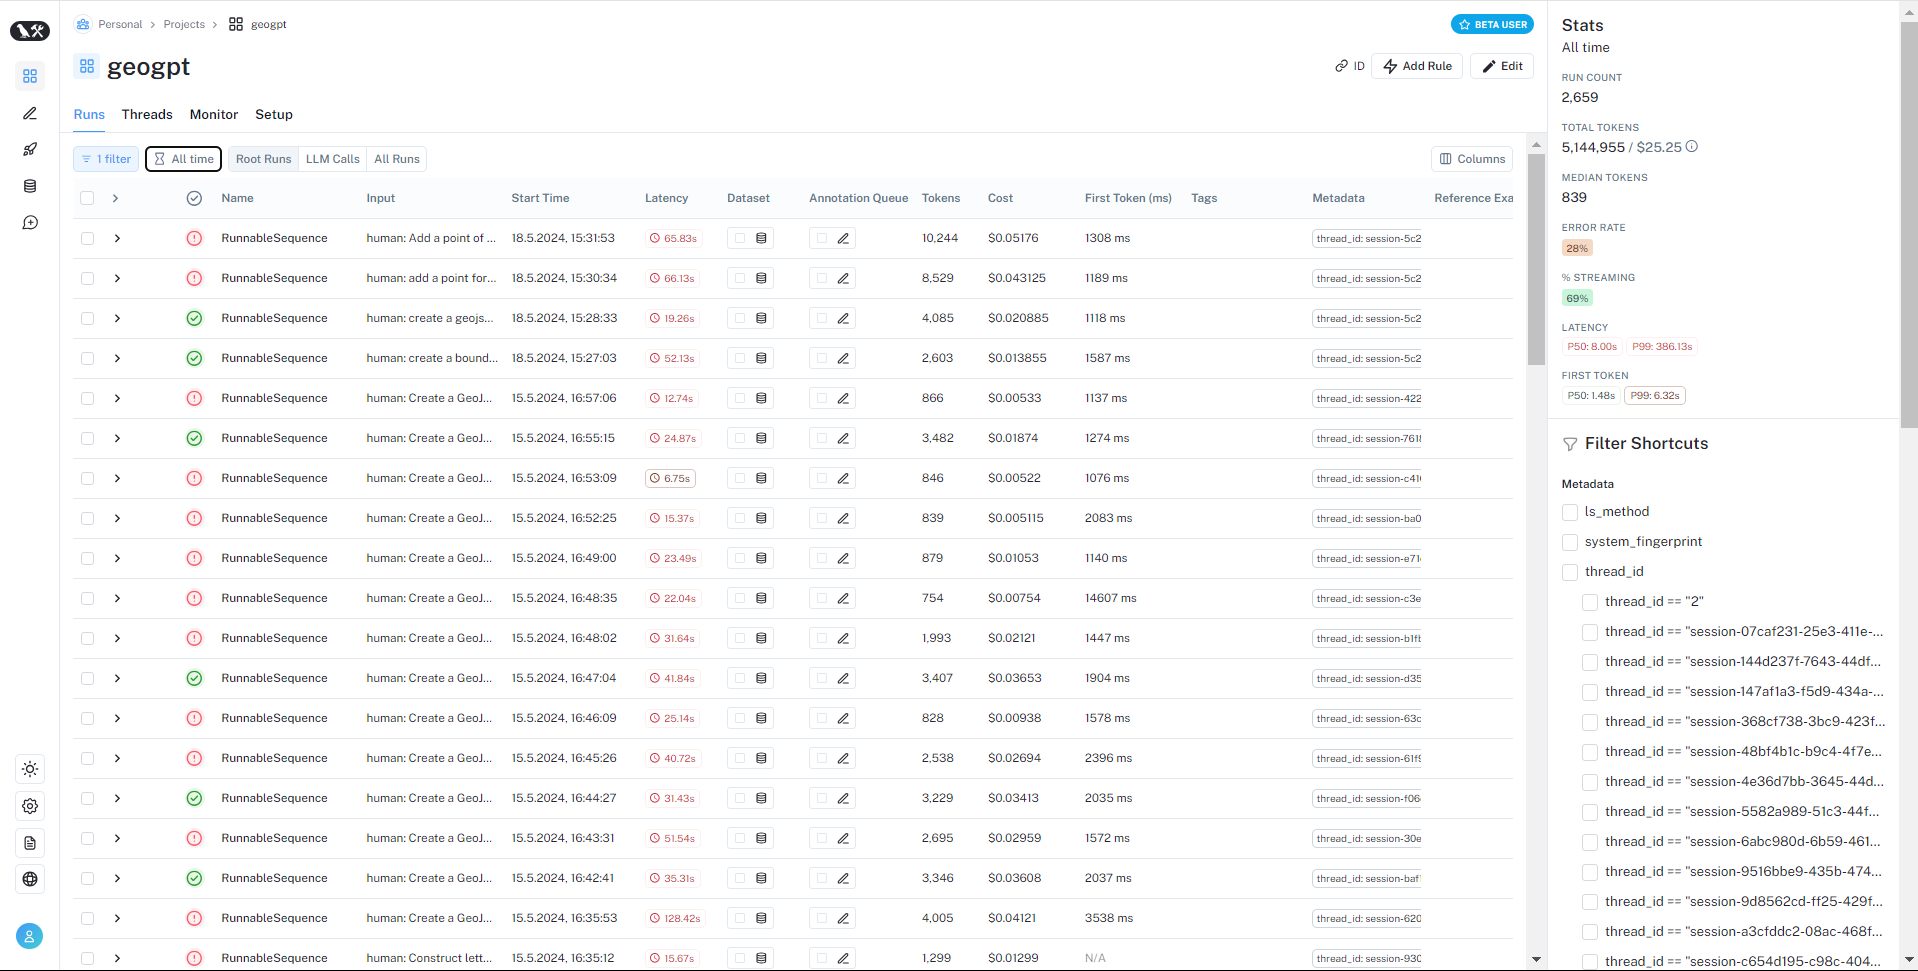
\includegraphics[width=\textwidth]{langsmith_main.png}
    %     \caption{Main page for a LangSmith project, in this case the \enquote{geogpt} project}
    %     \label{fig:langsmith-main}
    % \end{figure}

    % \begin{figure}
    %     \centering
    %     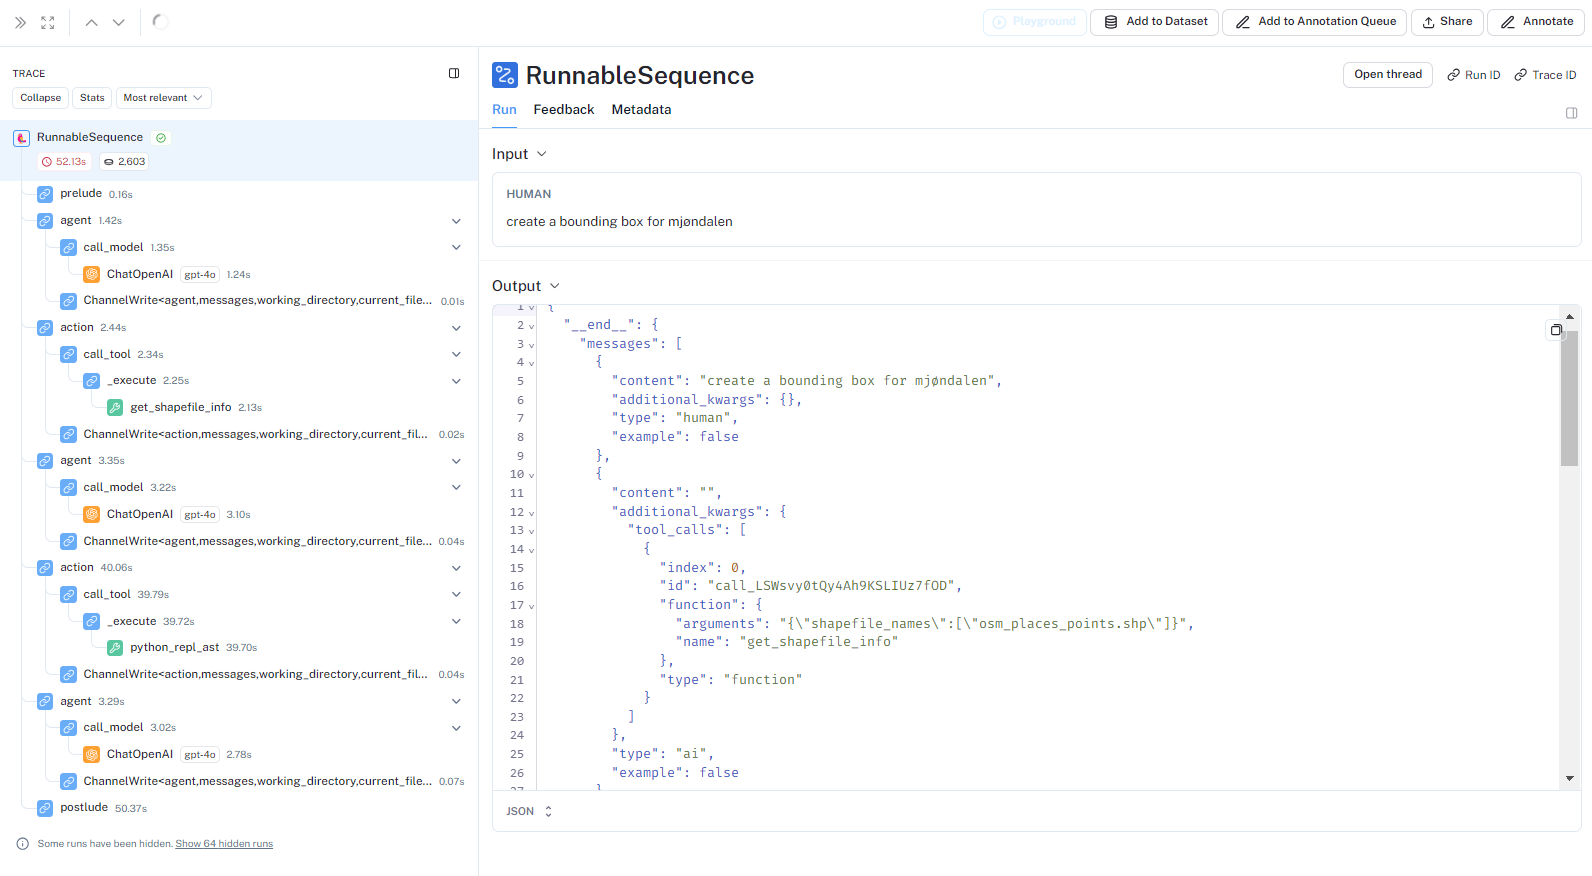
\includegraphics[width=\textwidth]{langsmith_trace.png}
    %     \caption{Trace for a given run of GeoGPT}
    %     \label{fig:langsmith-trace}
    % \end{figure}

    \begin{sidewaysfigure}
        \centering
        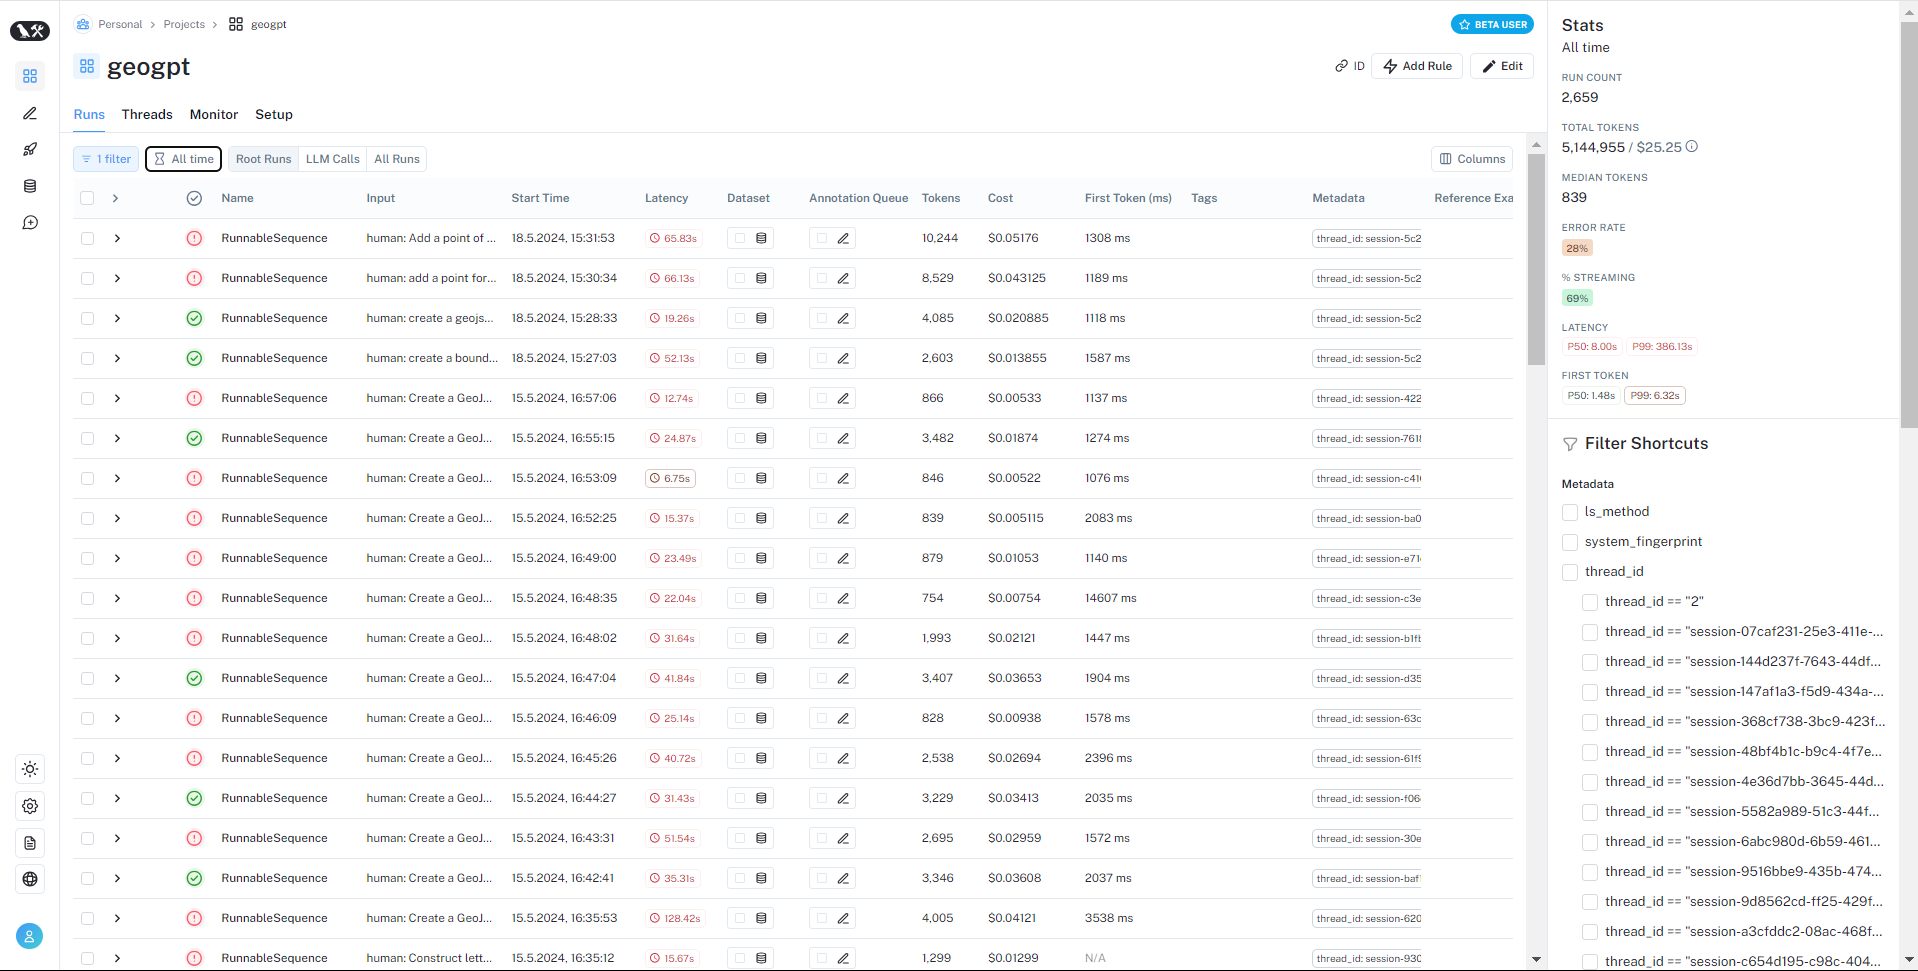
\includegraphics[width=\textwidth]{langsmith_main.png}
        \caption{Main page for a LangSmith project, in this case the \enquote{geogpt} project}
        \label{fig:langsmith-main}
    \end{sidewaysfigure}

    \begin{sidewaysfigure}
        \centering
        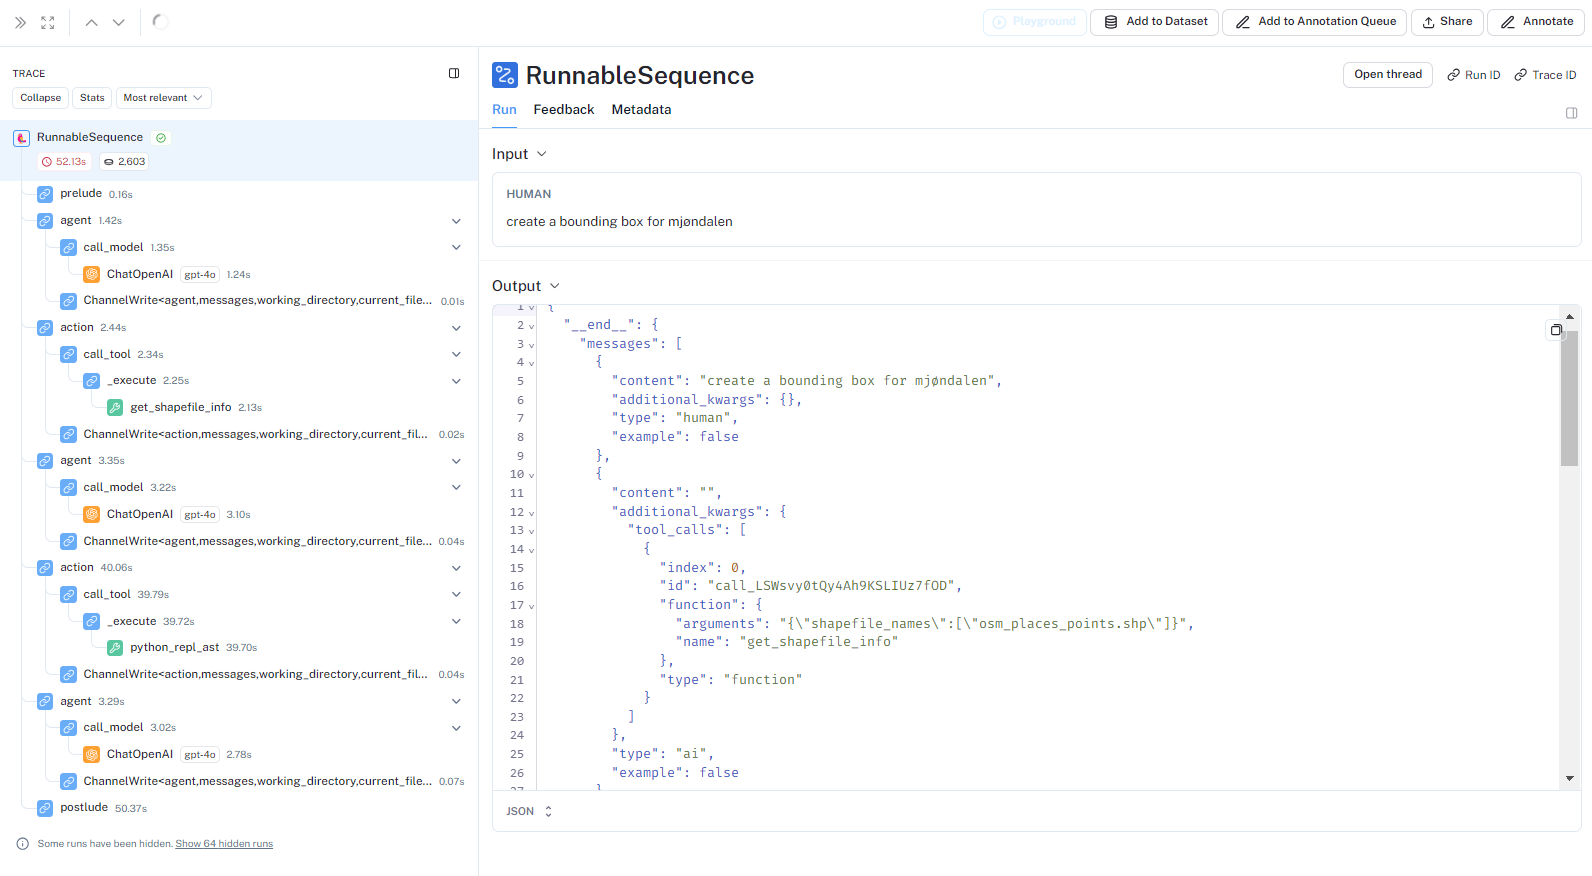
\includegraphics[width=\textwidth]{langsmith_trace.png}
        \caption{Trace for a given run of GeoGPT}
        \label{fig:langsmith-trace}
    \end{sidewaysfigure}



\end{appendix}